\chapter{Expanded Rigid Body Equations}
\section{Transformation of Linear Velocity}\label{sec:appendix-transformation-linvel}
\begin{align*}%
\begin{bmatrix}v_x \\ v_y \\ v_z\end{bmatrix}%
&=\begin{bmatrix}v_{x}^{CG} \\ v_{y}^{CG} \\ v_{z}^{CG}\end{bmatrix}%
+\begin{bmatrix}\dot{\phi} \\ \dot{\theta} \\ \dot{\psi}\end{bmatrix}\times\begin{bmatrix}r_x \\ r_y \\ r_z\end{bmatrix} \\%
&=\begin{bmatrix}v_{x}^{CG} \\ v_{y}^{CG} \\ v_{z}^{CG}\end{bmatrix}%
+\begin{bmatrix}\dot{\theta}r_z - \dot{\psi}r_y \\\dot{\psi}r_x - \dot{\phi}r_z \\\dot{\phi}r_y - \dot{\theta}r_x\end{bmatrix}%
\end{align*}

\section{Transformation of Linear Acceleration}\label{sec:appendix-transformation-linacc}
\begin{align*}%
\begin{bmatrix}a_x \\ a_y \\ a_z\end{bmatrix}%
&=\begin{bmatrix}a_{x}^{CG} \\ a_{y}^{CG} \\ a_{z}^{CG}\end{bmatrix}%
+\begin{bmatrix}\ddot{\phi} \\ \ddot{\theta} \\ \ddot{\psi}\end{bmatrix}\times\begin{bmatrix}r_x \\ r_y \\ r_z\end{bmatrix}%
+\begin{bmatrix}\dot{\phi} \\ \dot{\theta} \\ \dot{\psi}\end{bmatrix}\times \left(\begin{bmatrix}\dot{\phi} \\ \dot{\theta} \\ \dot{\psi}\end{bmatrix}\times\begin{bmatrix}r_x \\ r_y \\ r_z\end{bmatrix}\right)\\%
&=\begin{bmatrix}a_{x}^{CG} \\ a_{y}^{CG} \\ a_{z}^{CG}\end{bmatrix}%
+\begin{bmatrix}\ddot{\phi} \\ \ddot{\theta} \\ \ddot{\psi}\end{bmatrix}\times\begin{bmatrix}r_x \\ r_y \\ r_z\end{bmatrix}%
+\begin{bmatrix}\dot{\phi} \\ \dot{\theta} \\ \dot{\psi}\end{bmatrix}\times\begin{bmatrix}\dot{\theta}r_z - \dot{\psi}r_y \\\dot{\psi}r_x - \dot{\phi}r_z \\\dot{\phi}r_y - \dot{\theta}r_x\end{bmatrix}\\%
&=\begin{bmatrix}a_{x}^{CG} \\ a_{y}^{CG} \\ a_{z}^{CG}\end{bmatrix}%
+\begin{bmatrix}\ddot{\theta}r_z - \ddot{\psi}r_y \\\ddot{\psi}r_x - \ddot{\phi}r_z \\\ddot{\phi}r_y - \ddot{\theta}r_x\end{bmatrix}%
+\begin{bmatrix}\dot{\theta}(\dot{\phi}r_y - \dot{\theta}r_x) - \dot{\psi}(\dot{\psi}r_x - \dot{\phi}r_z)\\\dot{\psi}(\dot{\theta}r_z - \dot{\psi}r_y) - \dot{\phi}(\dot{\phi}r_y - \dot{\theta}r_x)\\\dot{\phi}(\dot{\psi}r_x - \dot{\phi}r_z) - \dot{\theta}(\dot{\theta}r_z - \dot{\psi}r_y)\end{bmatrix}%
\end{align*}

\chapter{Extended Kalman Filter Equations}\label{sec:appendix-ekf-equations}

\section{Jacobian of Process Function With Respect to State Vector}
\begin{equation*}%
\frac{\partial \dot{x}}{\partial x} = \begin{bmatrix}%
0 & 0 & cos(\psi) & -sin(\psi) & -v_x \cdot sin(\psi) - v_y \cdot cos(\psi) & 0 \\%
0 & 0 & sin(\psi) & cos(\psi) & v_x \cdot cos(\psi) - v_y \cdot sin(\psi) & 0 \\%
0 & 0 & 0 & \dot{\psi} & 0 & v_y \\%
0 & 0 & -\dot{\psi} & 0 & 0 & -v_x \\%
0 & 0 & 0 & 0 & 0 & 1 \\%
0 & 0 & 0 & 0 & 0 & 0%
\end{bmatrix}%
\end{equation*}

\section{Jacobian of Process Function With Respect to Input Vector}
\begin{equation*}%
\frac{\partial \dot{x}}{\partial u} = \begin{bmatrix}%
0 & 0 & 0 \\%
0 & 0 & 0 \\%
1 & 0 & 0 \\%
0 & 1 & 0 \\%
0 & 0 & 0 \\%
0 & 0 & 1%
\end{bmatrix}%
\end{equation*}

\section{Measurement Matrix}\label{sec:appendix-ekf-measurement}
\begin{equation*}%
H = \begin{bmatrix}%
1 & 0 & 0 & 0 & 0 & 0 \\%
0 & 1 & 0 & 0 & 0 & 0 \\%
0 & 0 & 1 & 0 & 0 & 0 \\%
0 & 0 & 0 & 1 & 0 & 0 \\%
0 & 0 & 1 & 0 & 0 & 0 \\%
0 & 0 & 1 & 0 & 0 & 0 \\%
0 & 0 & 0 & 0 & 1 & 0 \\%
0 & 0 & 0 & 0 & 0 & 1%
\end{bmatrix}%
\end{equation*}

\chapter{Evaluation Results}

\section{IMU Fusion}\label{sec:appendix-imufusion}
\subsection{Raw Data From Front IMU}
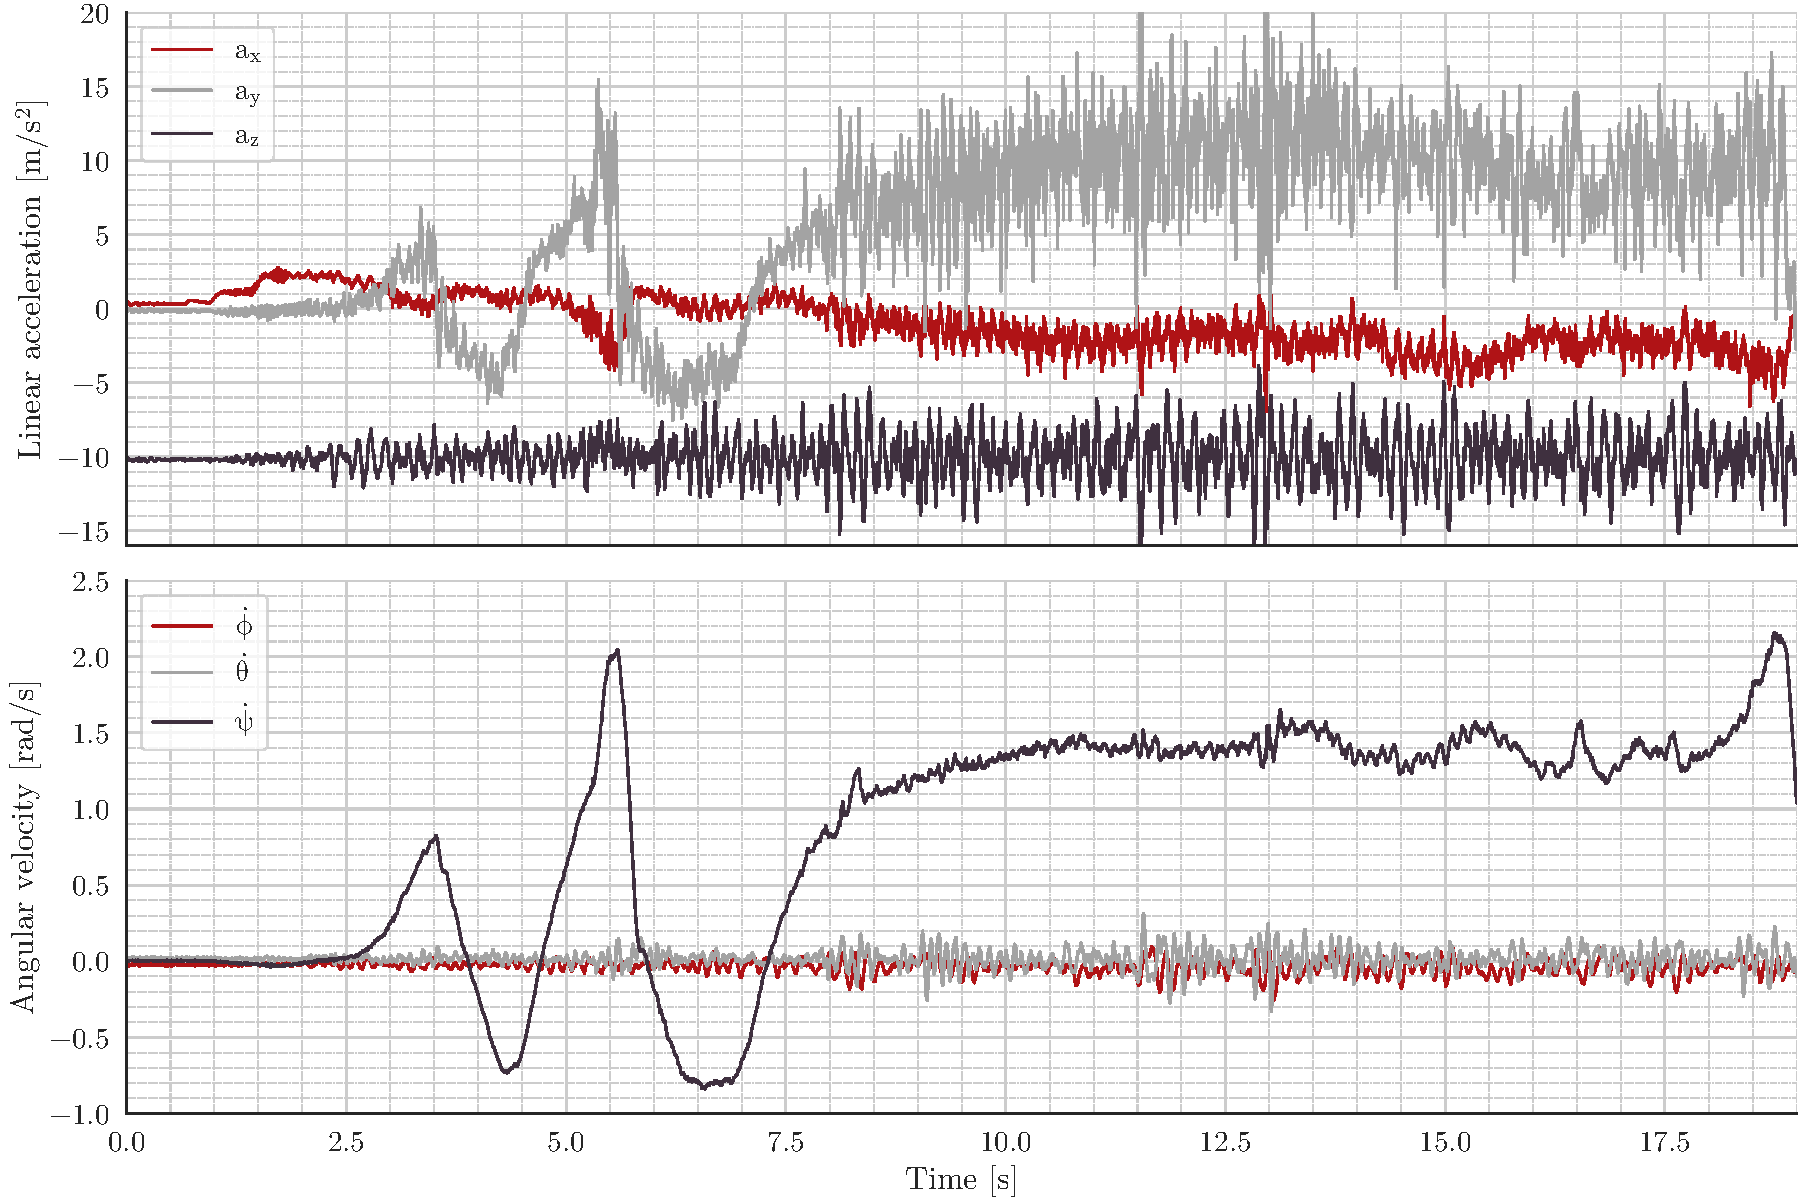
\includegraphics[width=\textwidth]{plot_imu_fusion_full_imu1}
\subsection{Raw Data From Rear IMU}
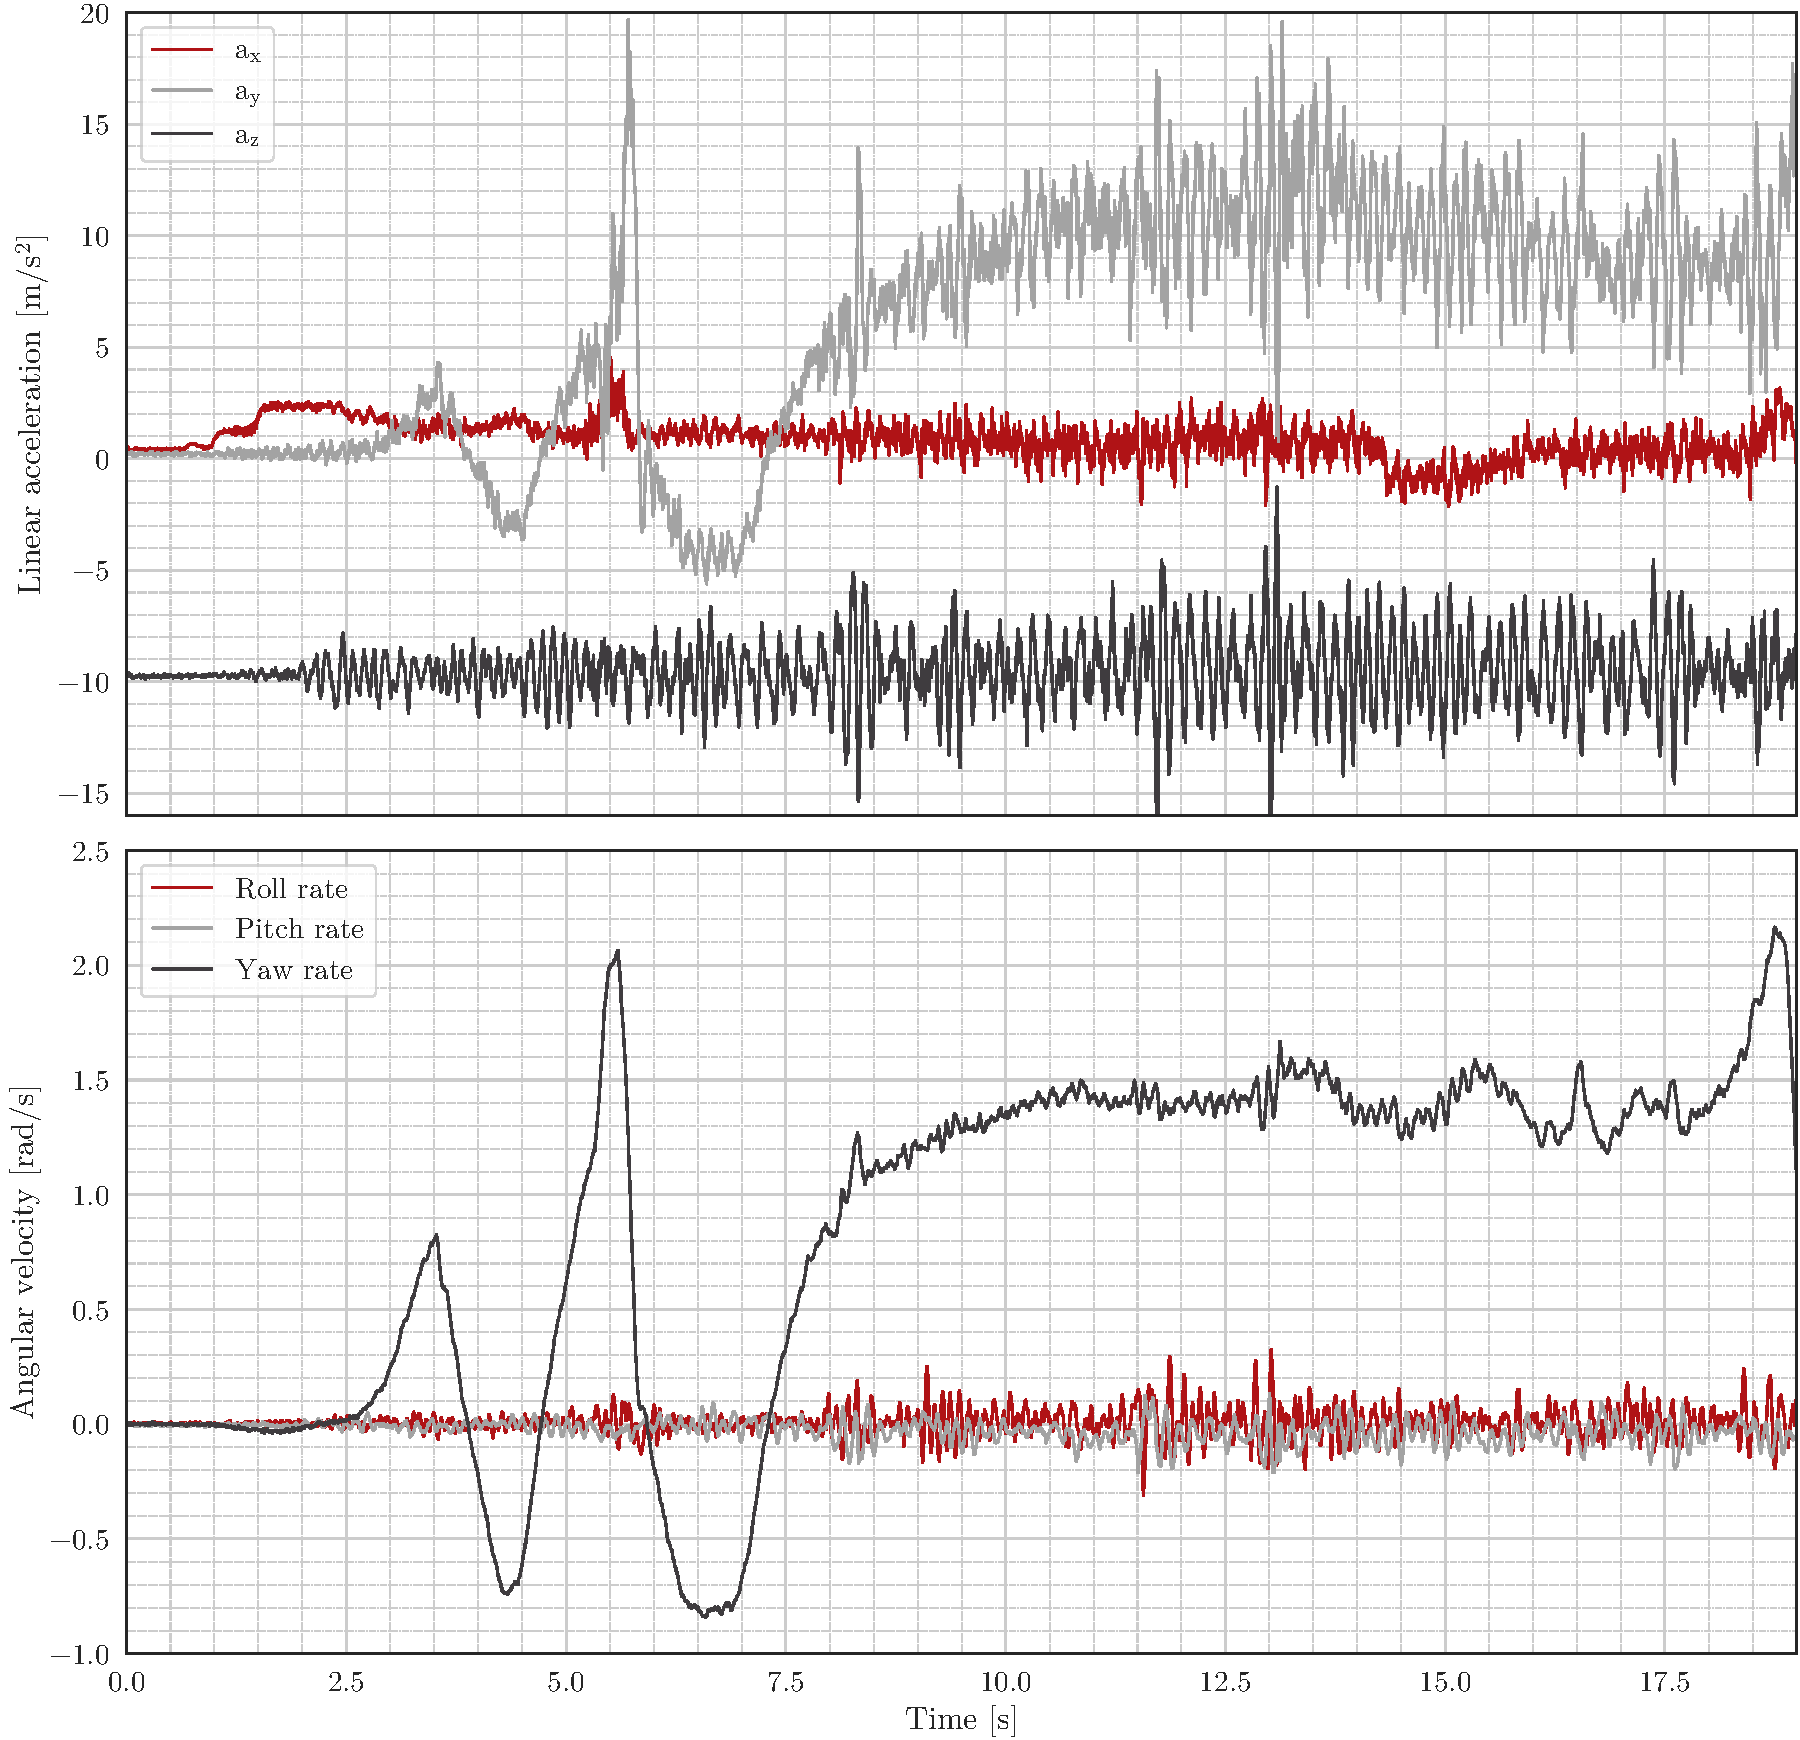
\includegraphics[width=\textwidth]{plot_imu_fusion_full_imu2}
\subsection{Fused Data With Mean-Based-Fusion}
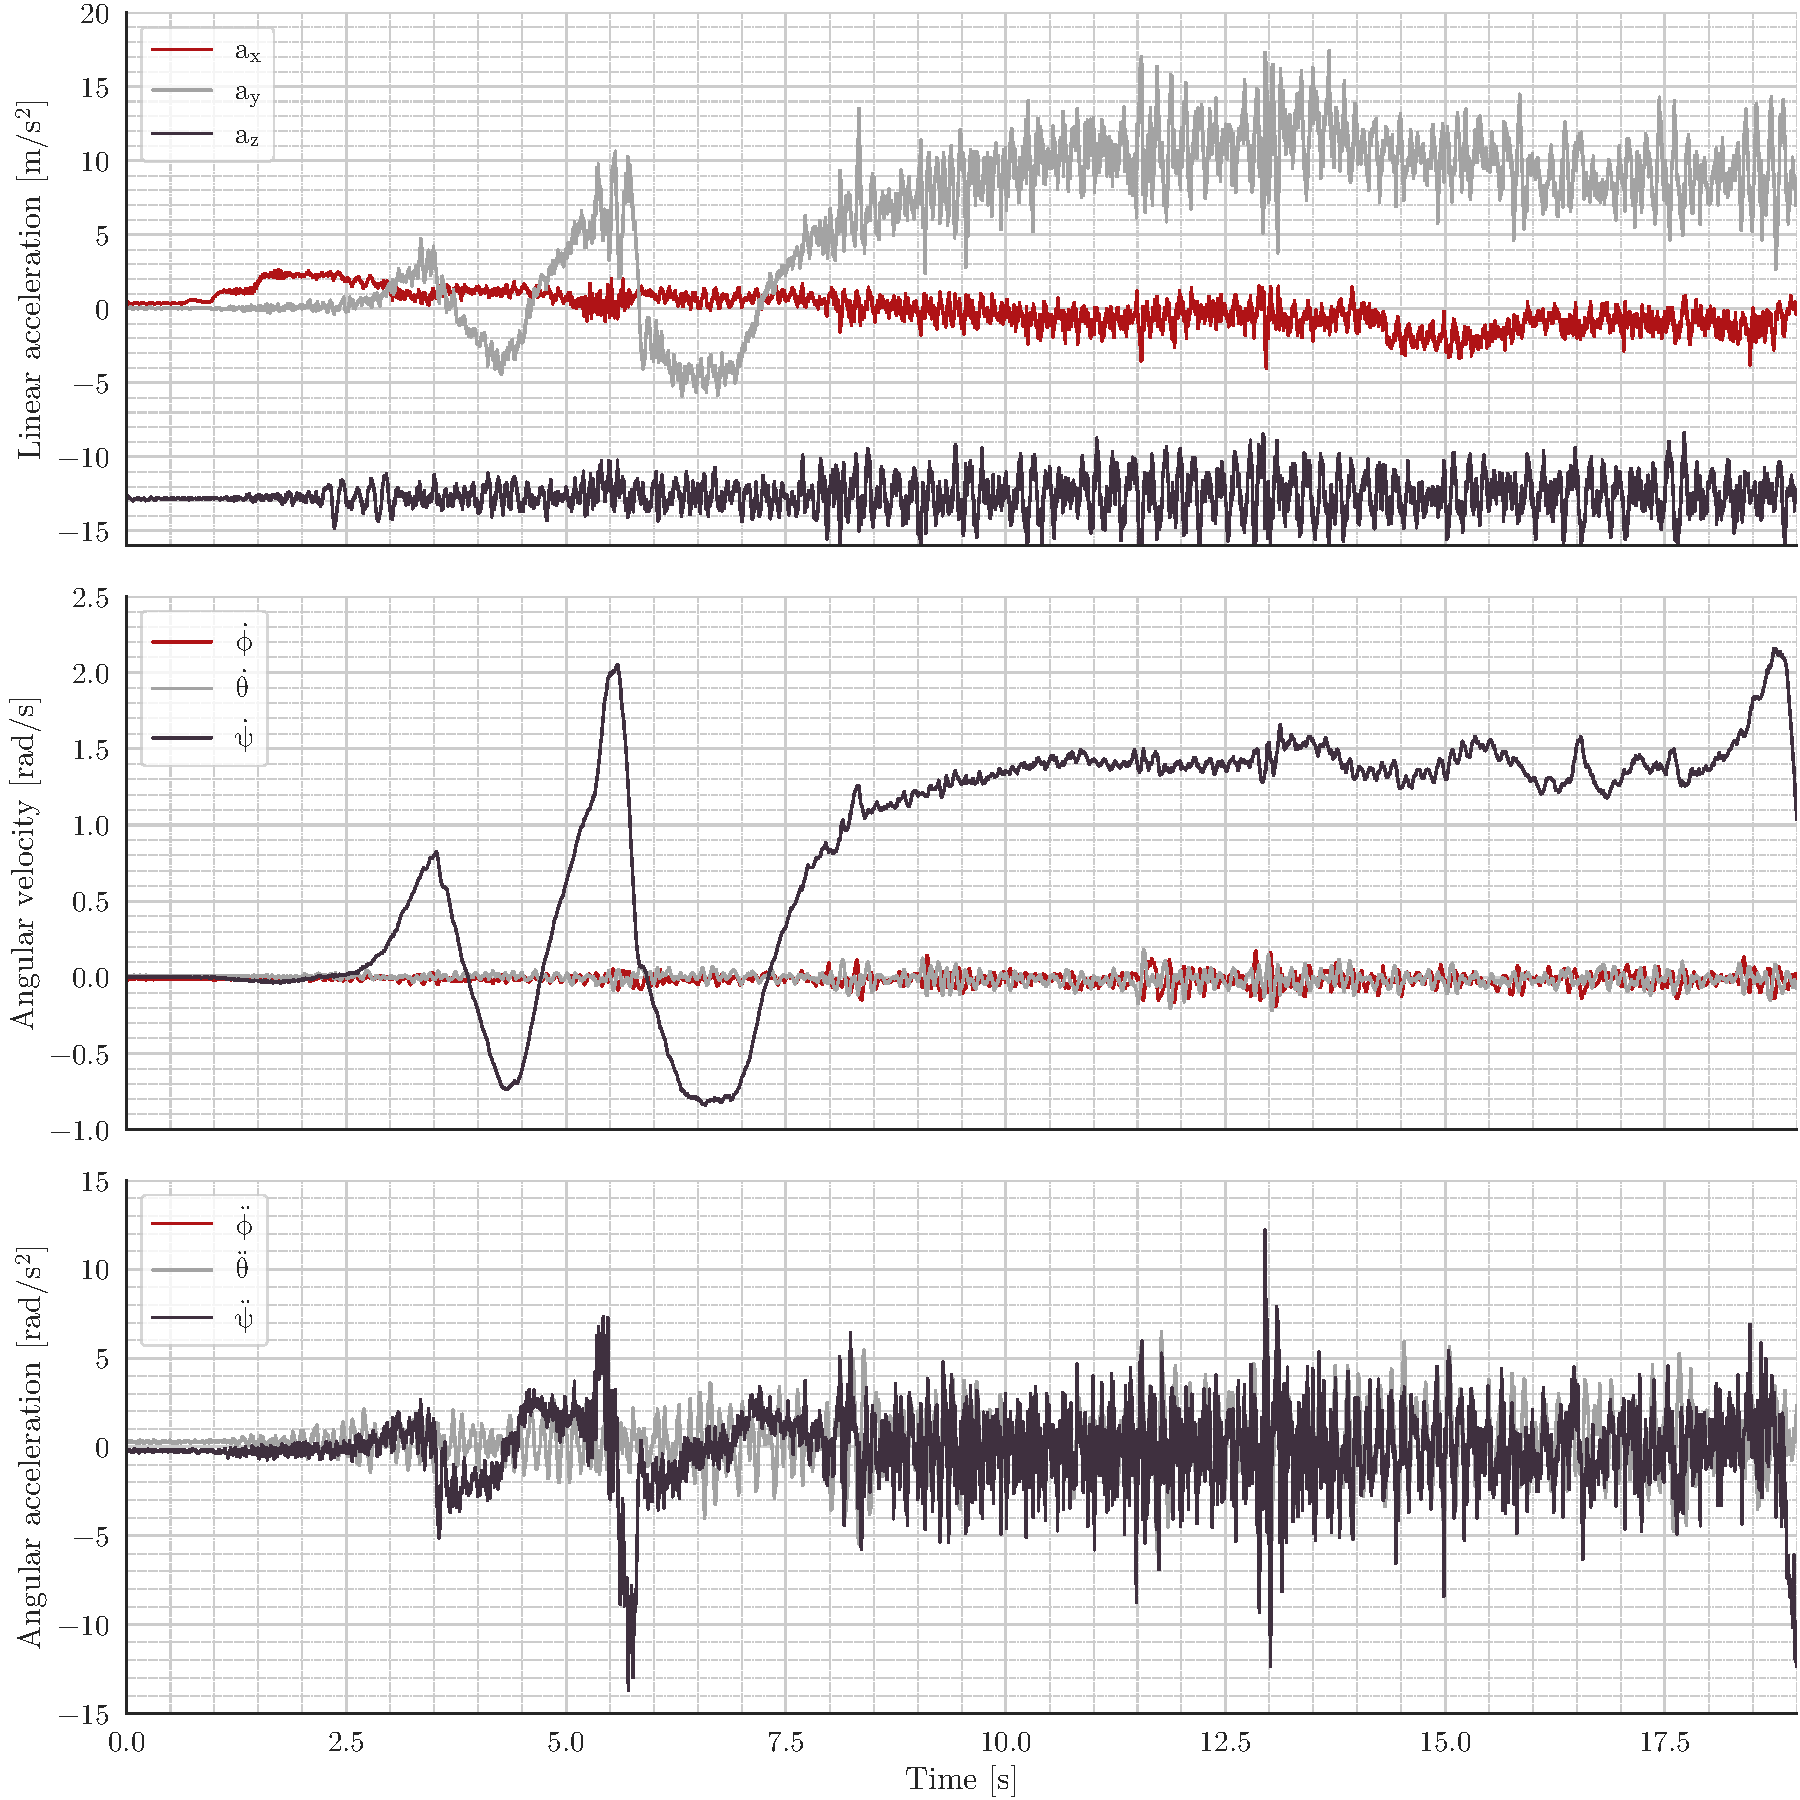
\includegraphics[width=\textwidth]{plot_imu_fusion_full_mean}
\subsection{Fused Data With Maximum-Likelihood-Based Fusion}
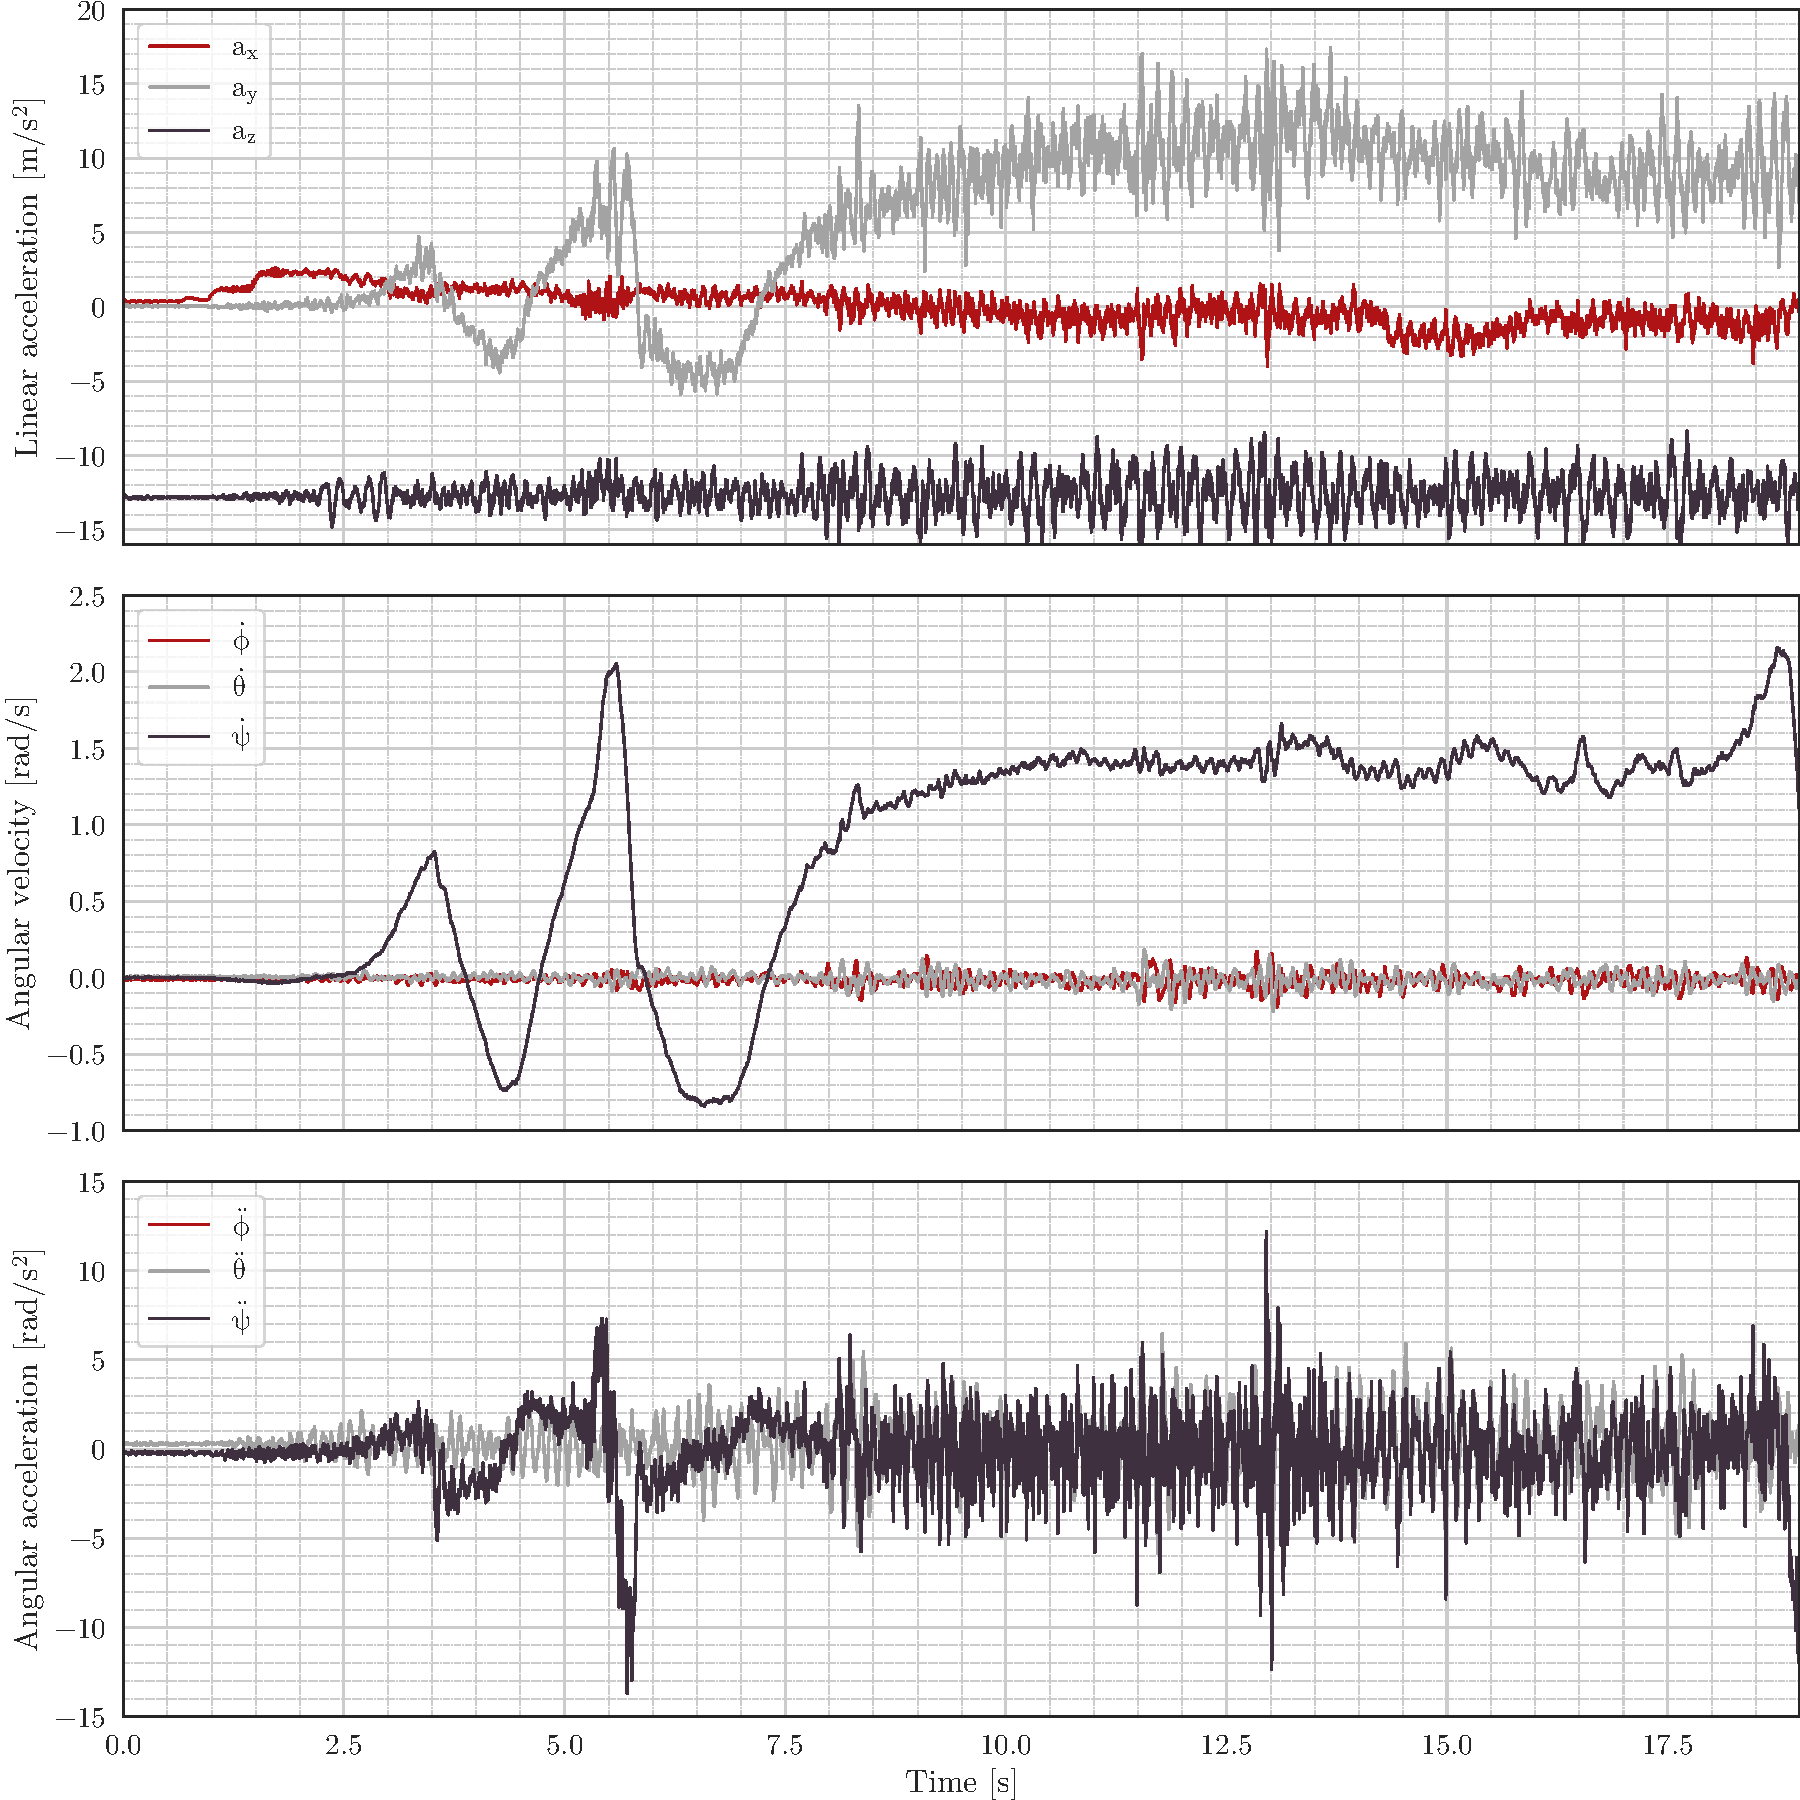
\includegraphics[width=\textwidth]{plot_imu_fusion_full_ls}

\section{Failure Detection}\label{sec:appendix-failure-detection}
\subsection{EKF Bank Residual Analysis}
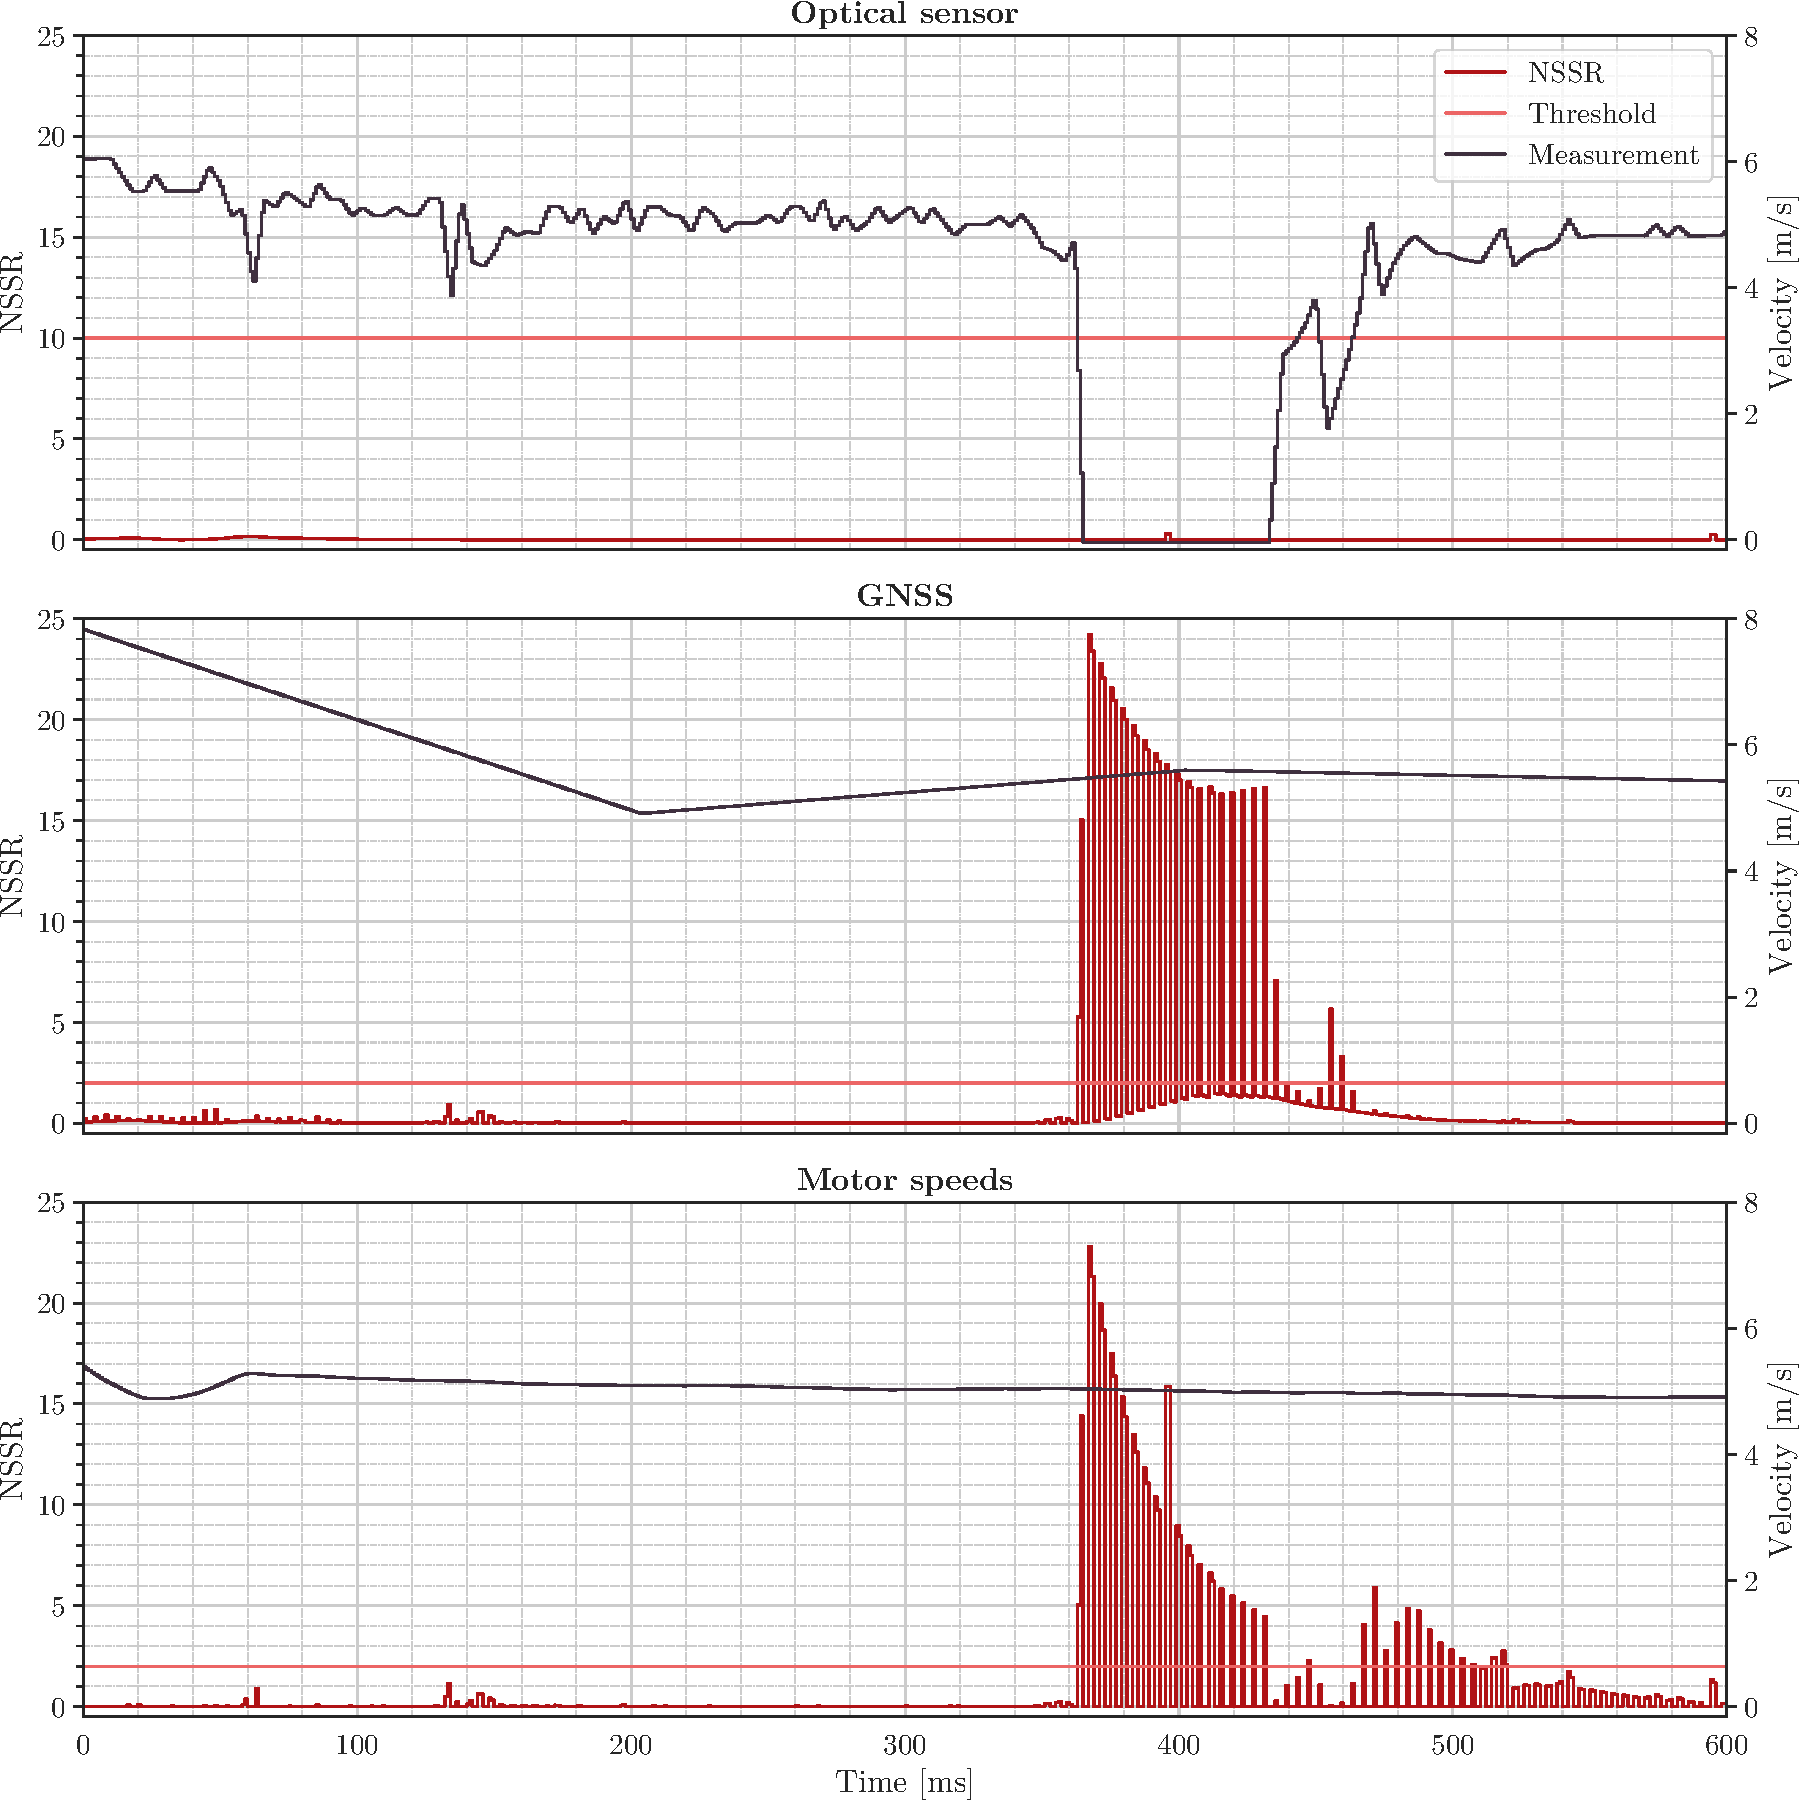
\includegraphics[width=\textwidth]{plot_failure_detection_nssr_full}

\section{EKF Estimates and Residuals}\label{sec:appendix-ekf}
\subsection{Position from GNSS without initial heading}
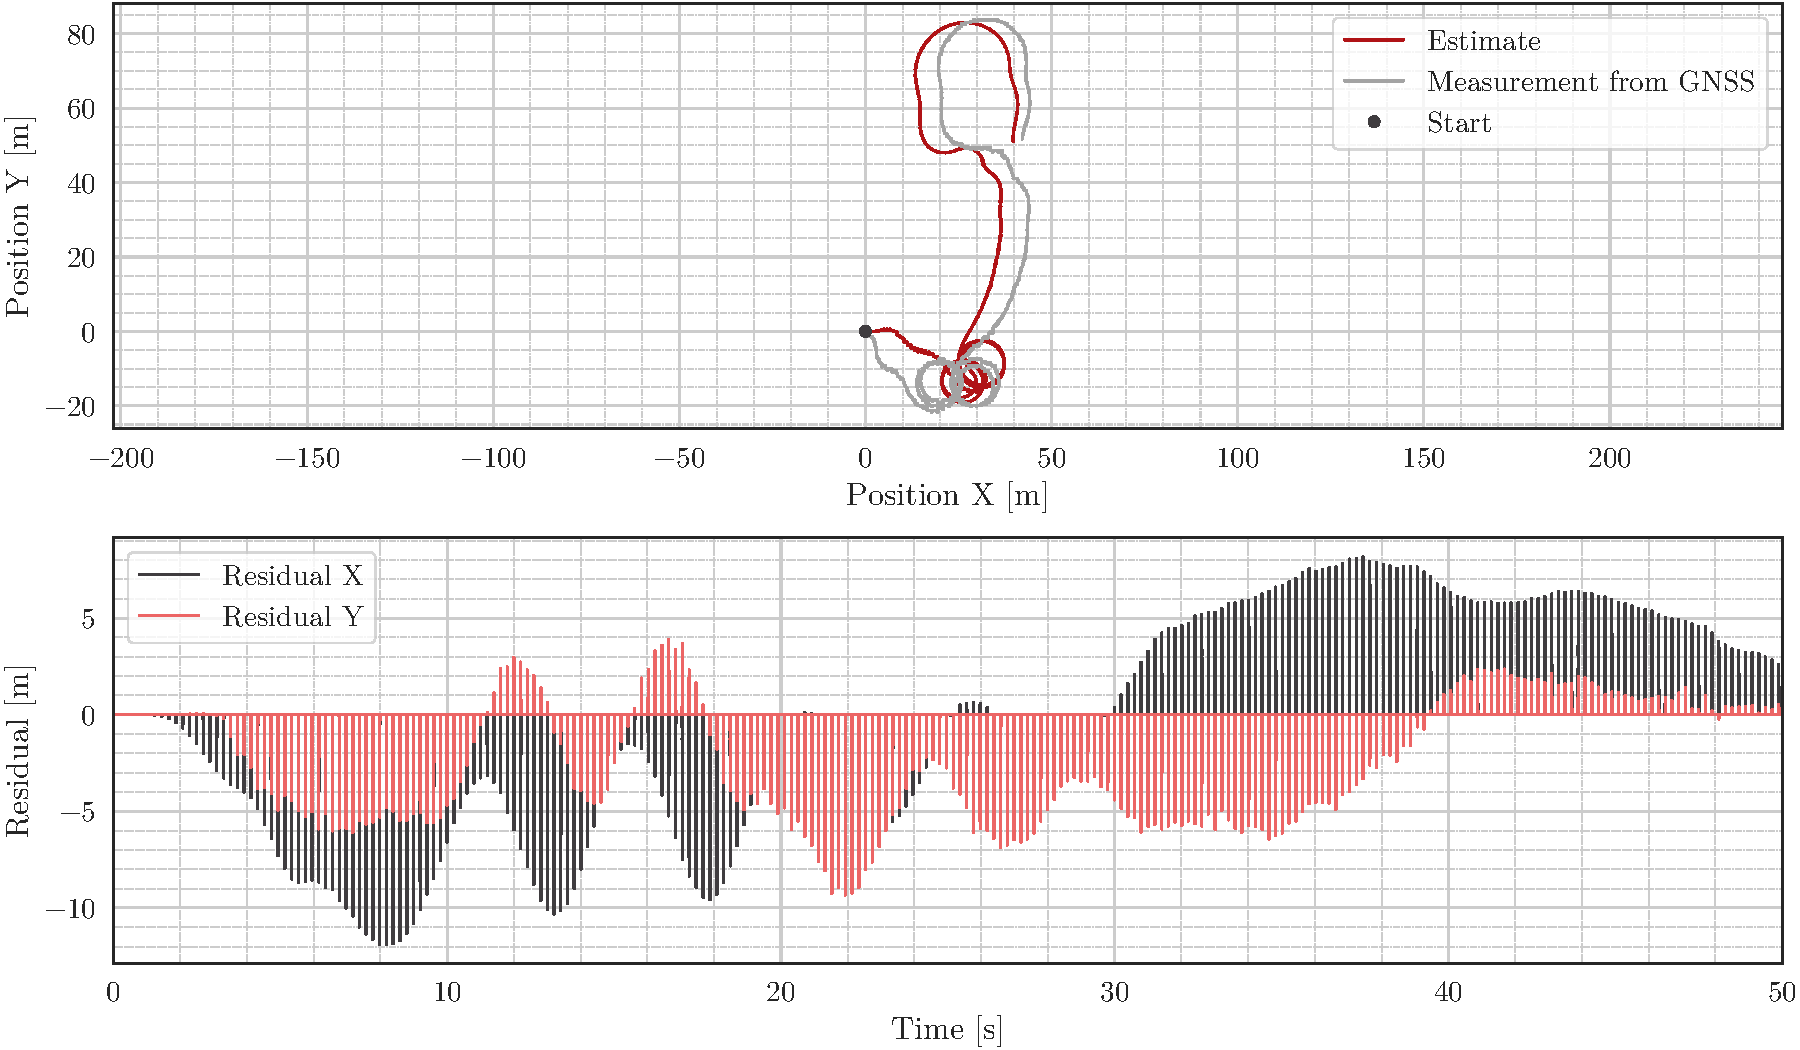
\includegraphics[width=\textwidth]{plot_ekf_full_xy_noheading}
\subsection{Position from GNSS with initial heading}
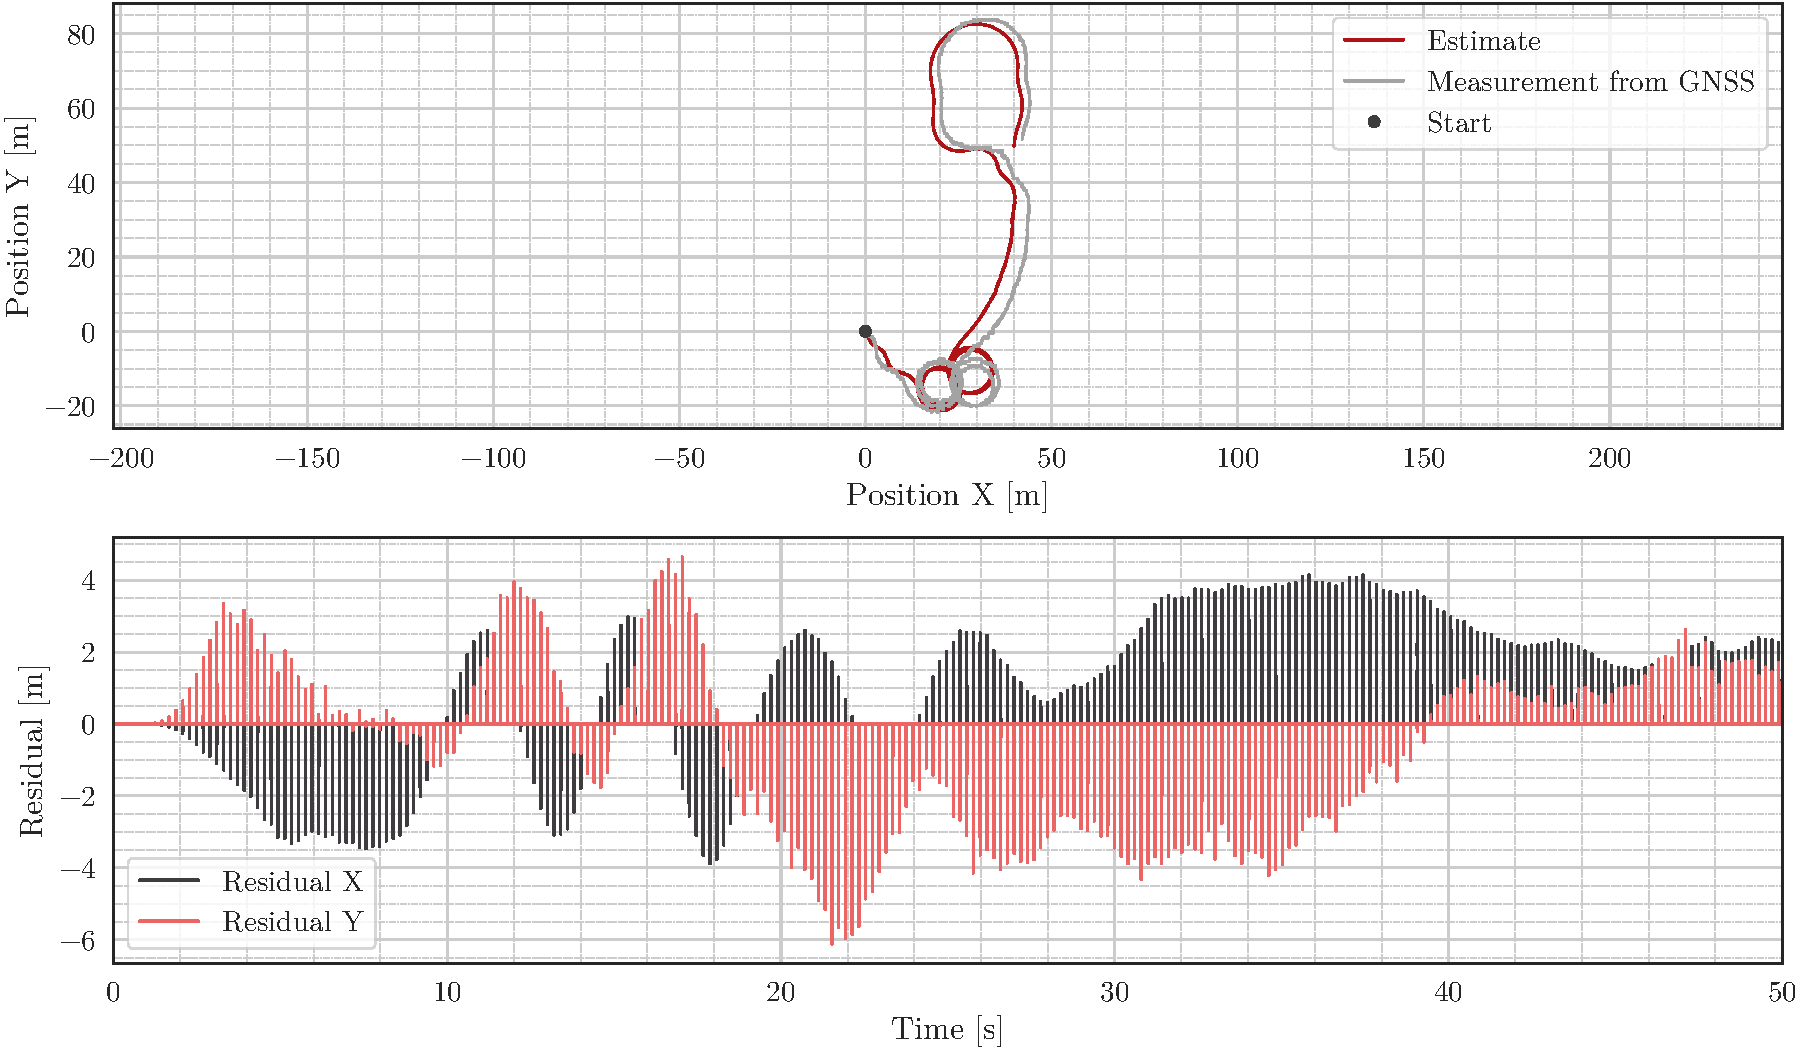
\includegraphics[width=\textwidth]{plot_ekf_full_xy_heading}
\subsection{Longitudinal velocity from optical sensor}
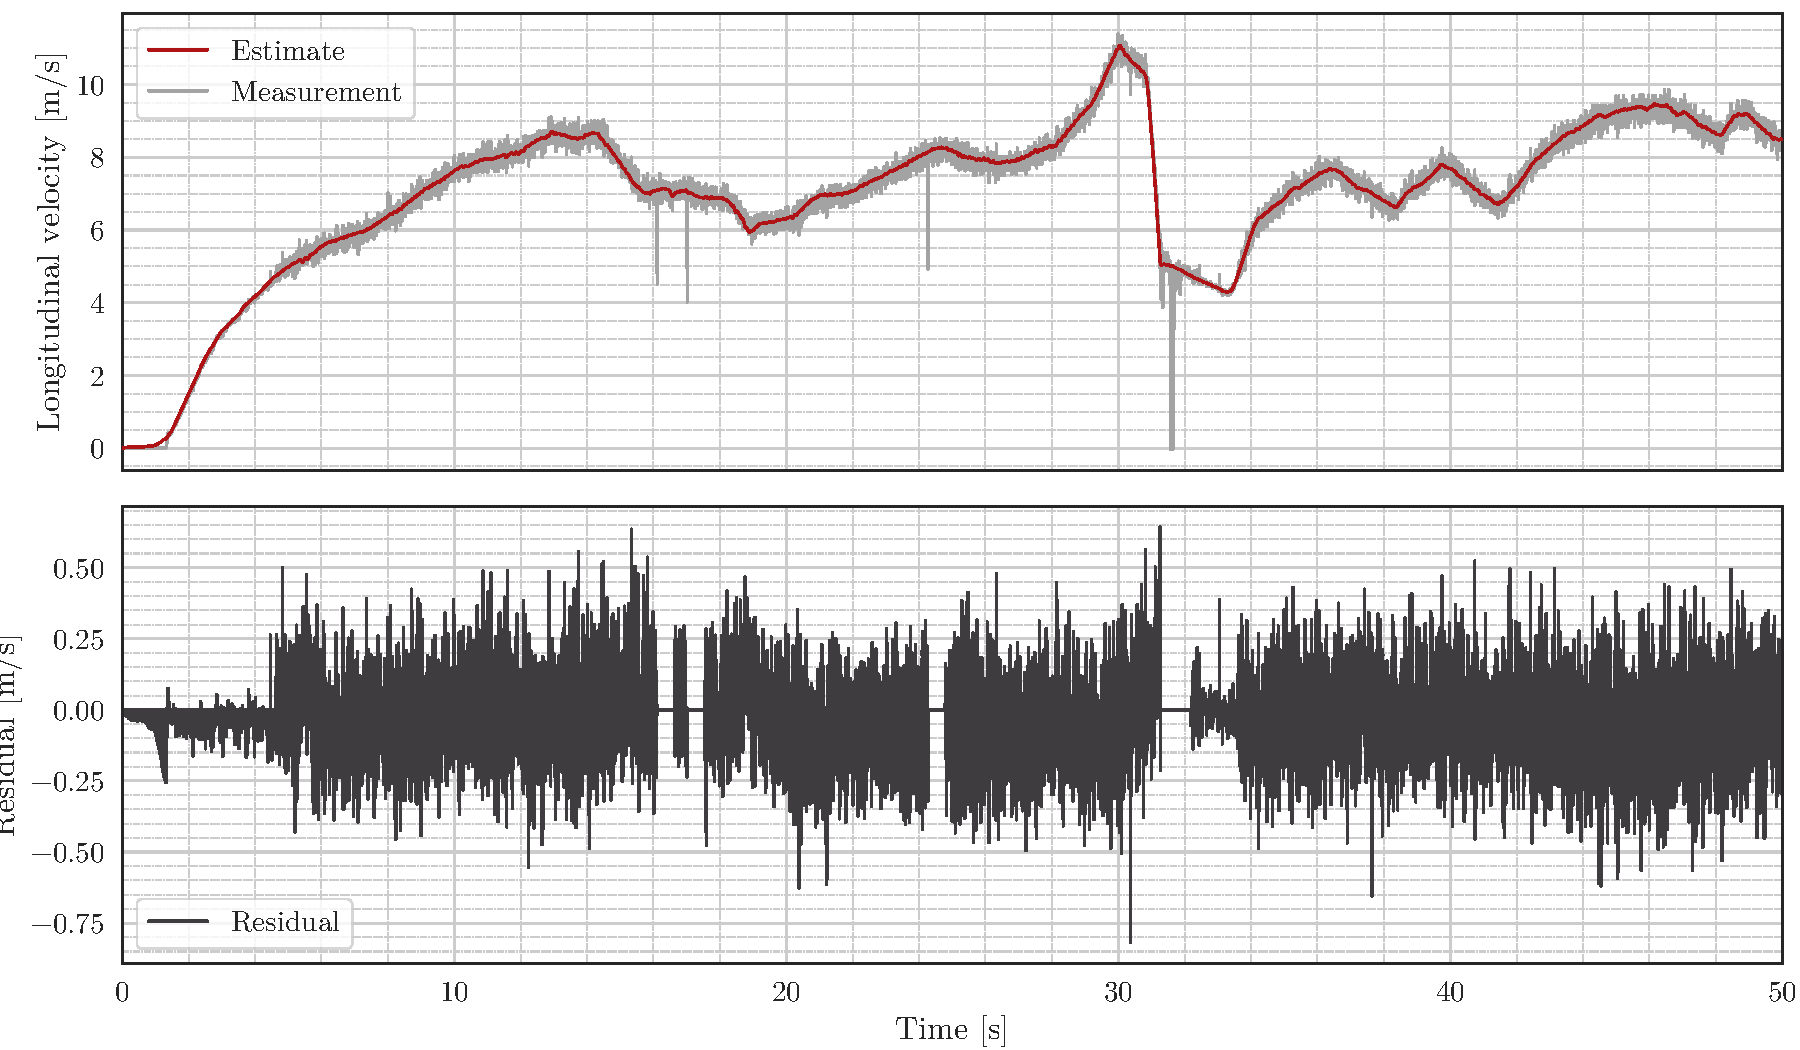
\includegraphics[width=\textwidth]{plot_ekf_full_vx_sfii}
\subsection{Lateral velocity from optical sensor}
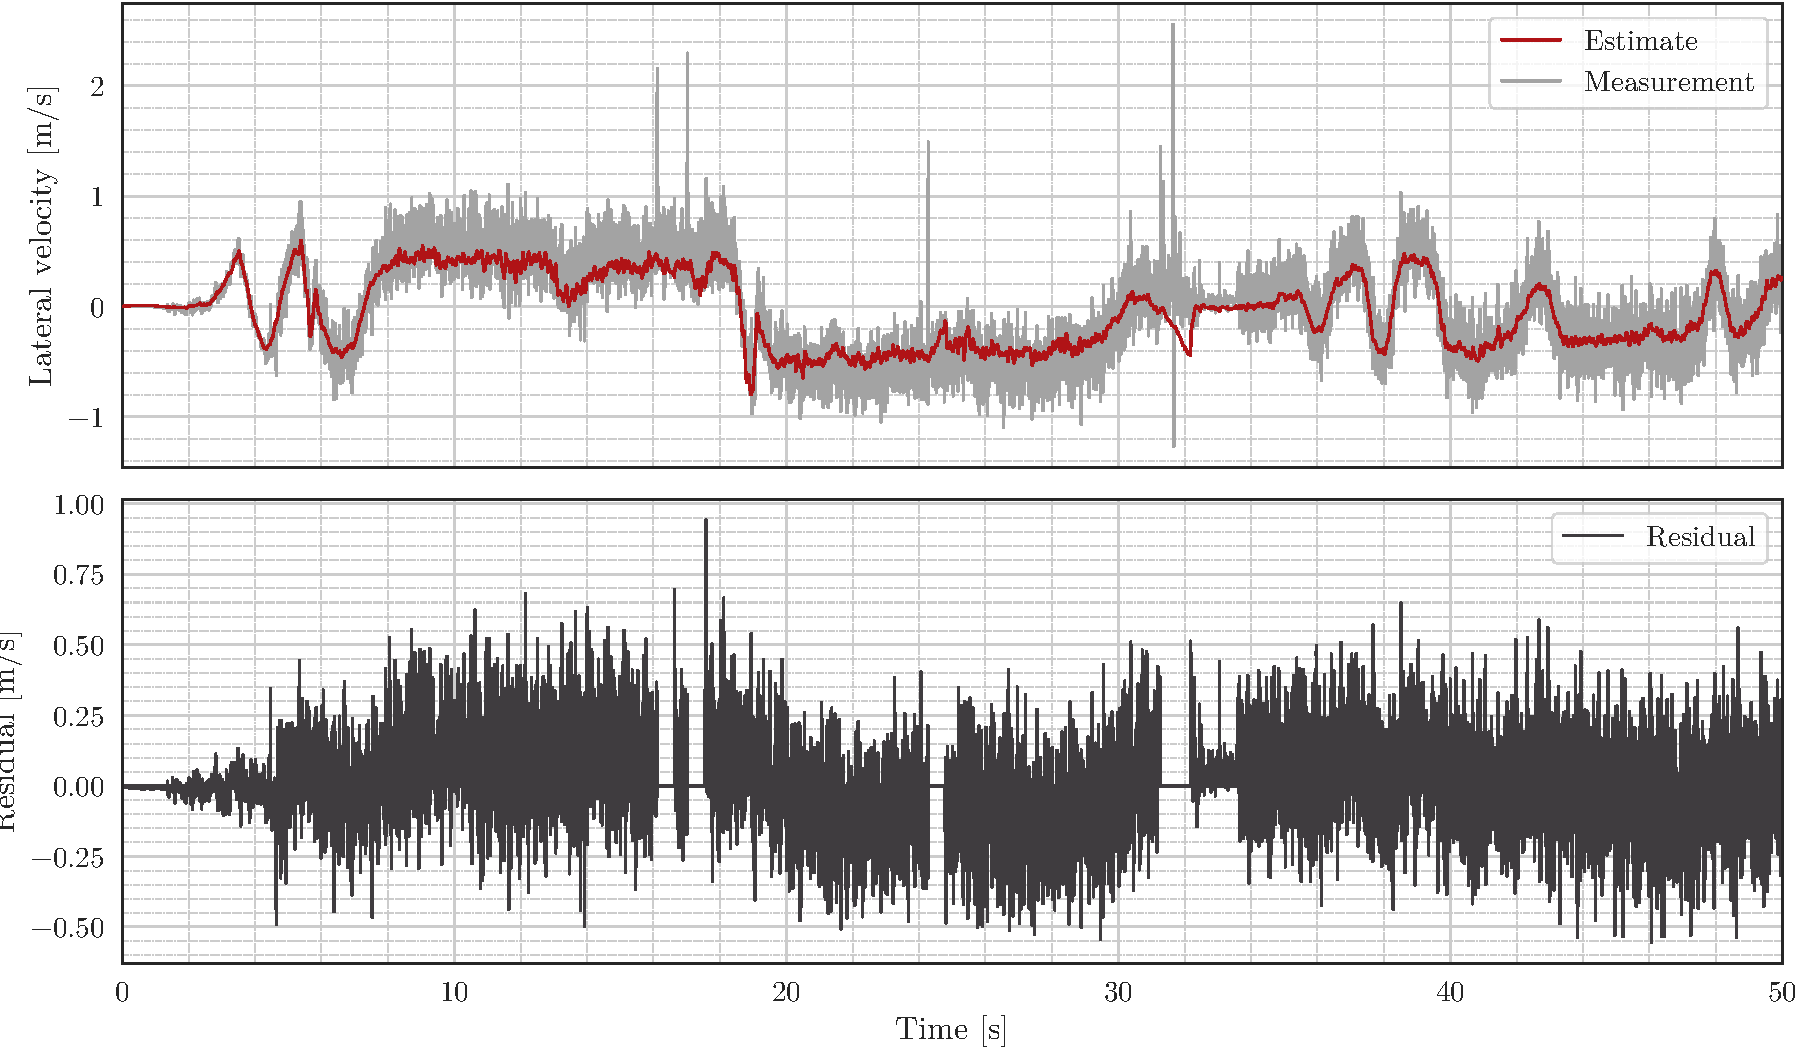
\includegraphics[width=\textwidth]{plot_ekf_full_vy_sfii}
\subsection{Longitudinal velocity from GNSS}
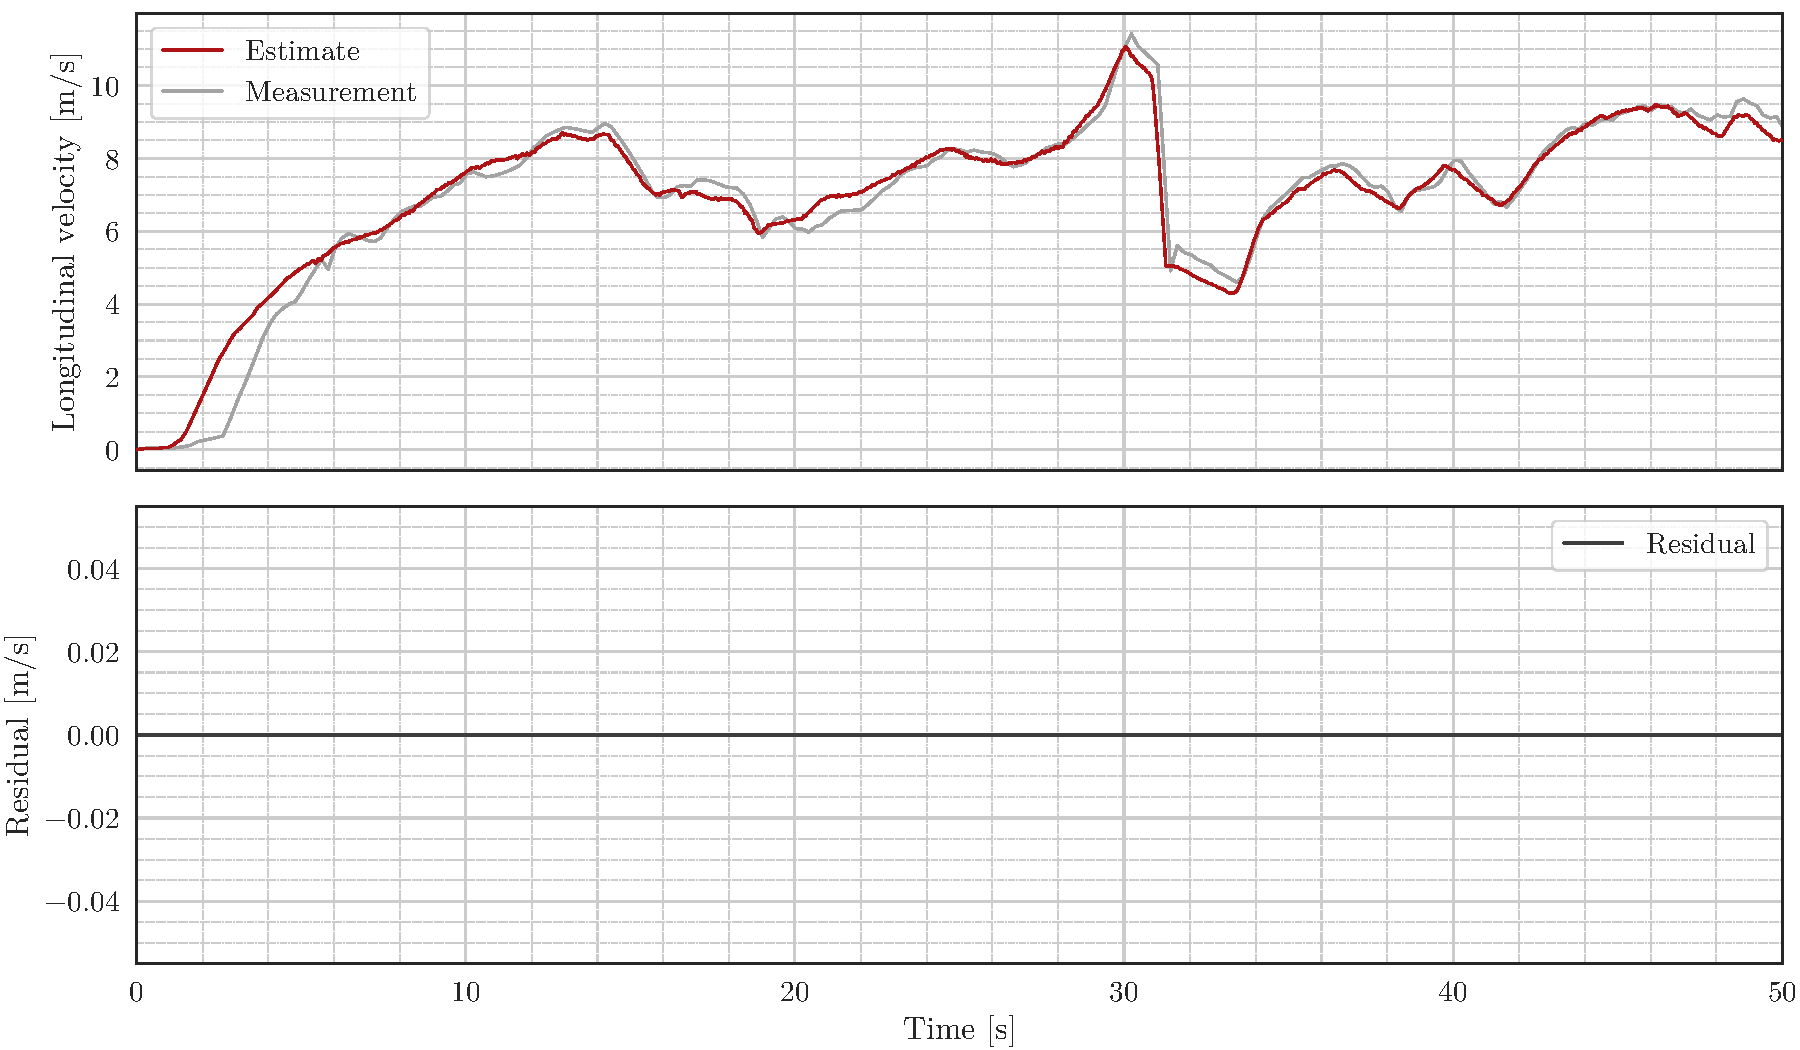
\includegraphics[width=\textwidth]{plot_ekf_full_vx_gps}
The \gls{gnss} velocity measurement is not used during normal operation, therefore it does not influence the estimate and residuals are zero.
\subsection{Longitudinal velocity from motor speeds}
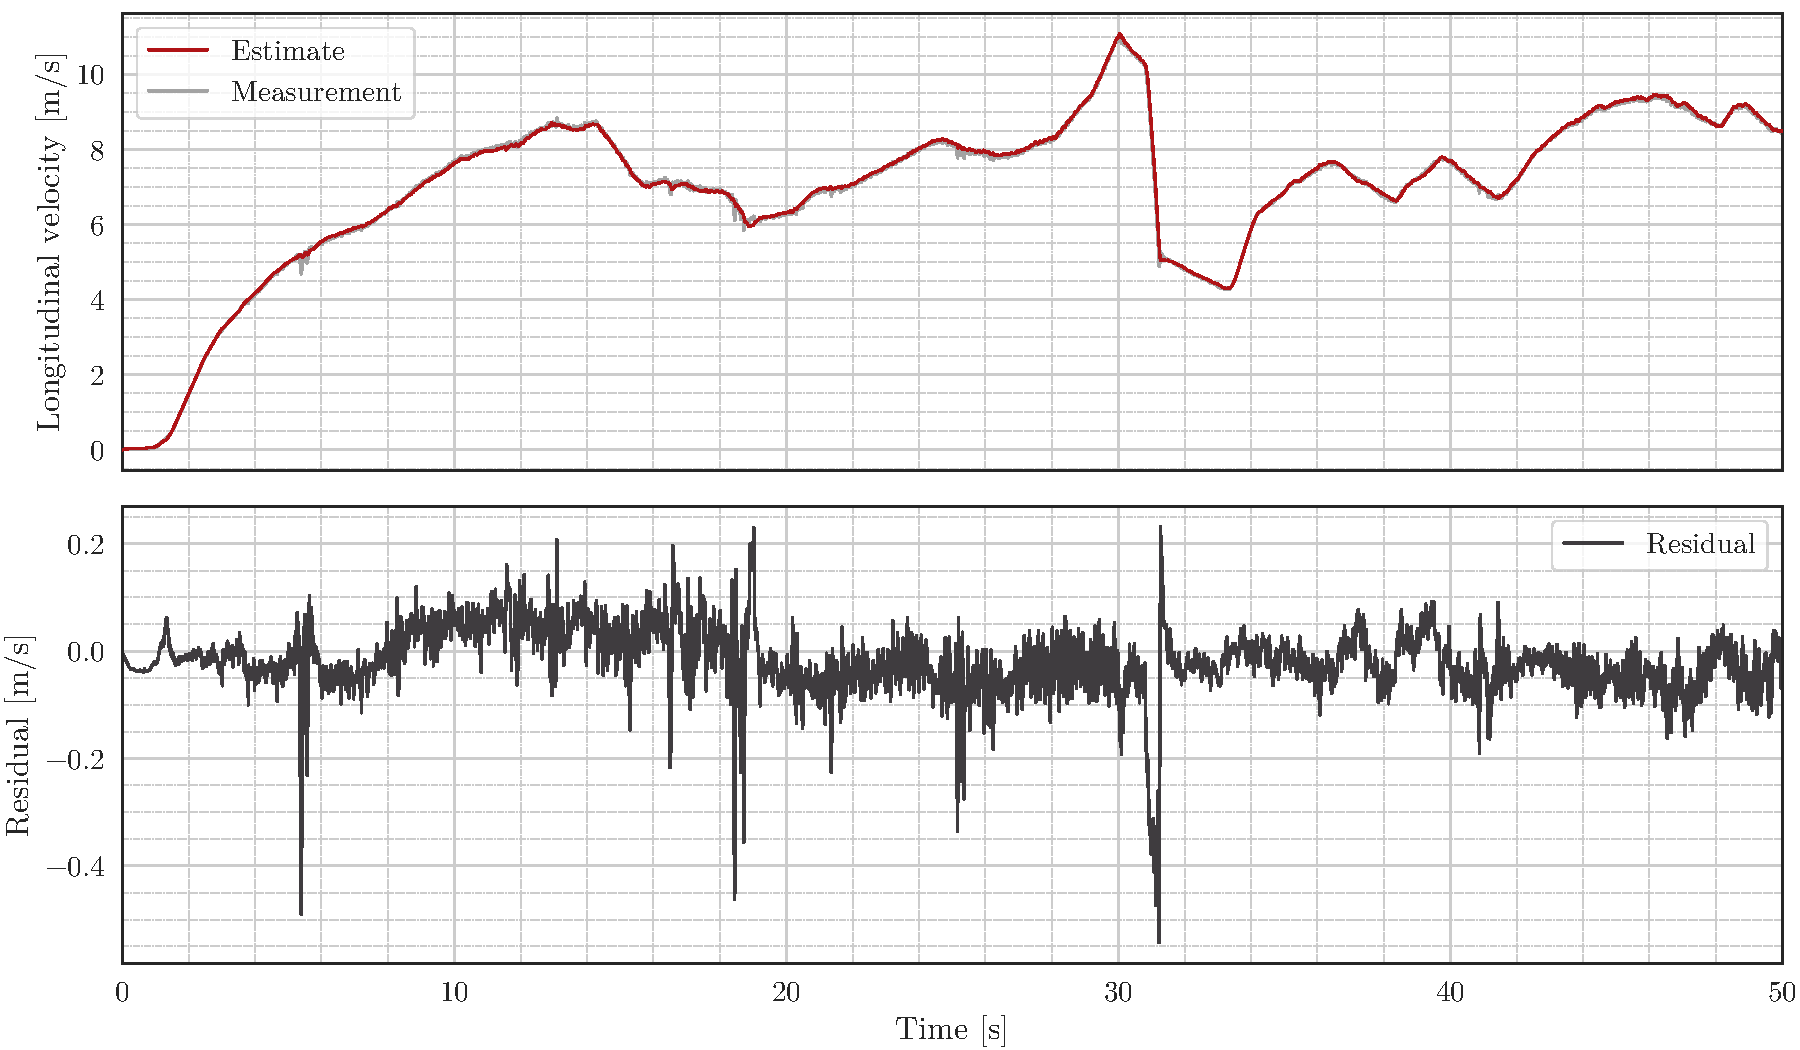
\includegraphics[width=\textwidth]{plot_ekf_full_vx_wheels}
\subsection{Heading from GNSS without initial heading}
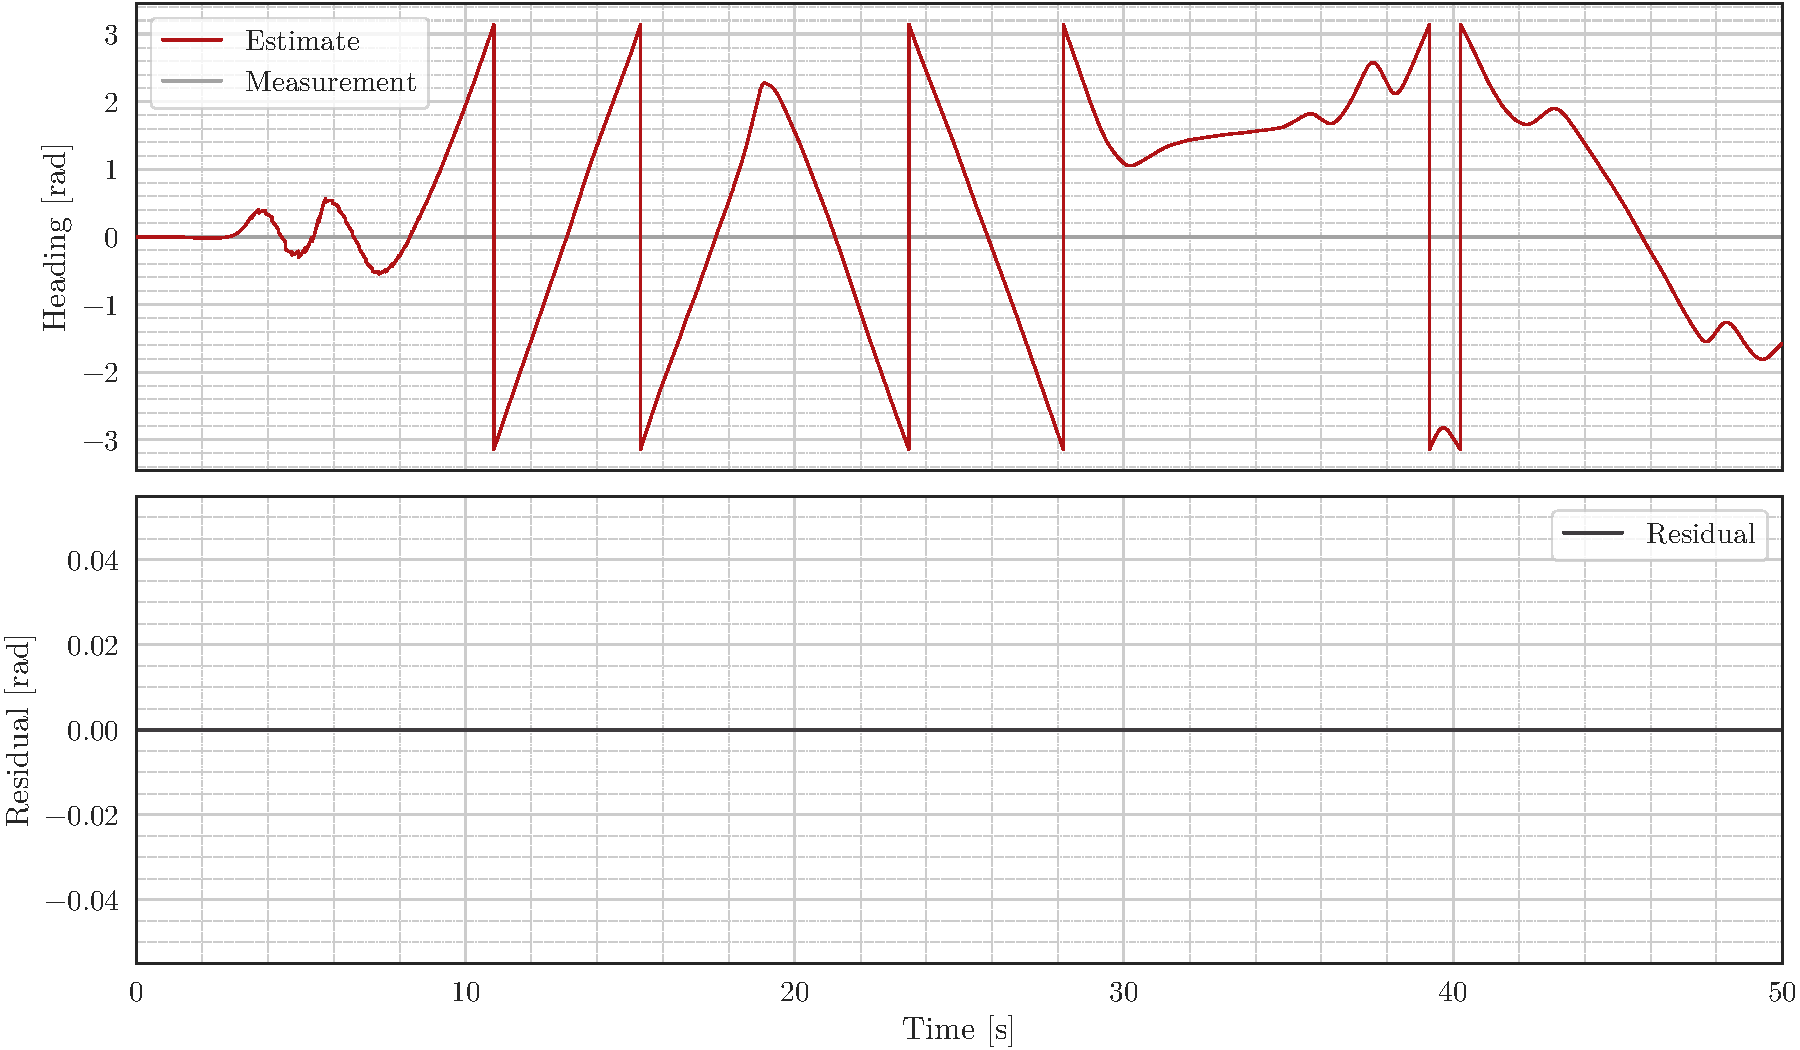
\includegraphics[width=\textwidth]{plot_ekf_full_psi}
\subsection{Heading from GNSS with initial heading}
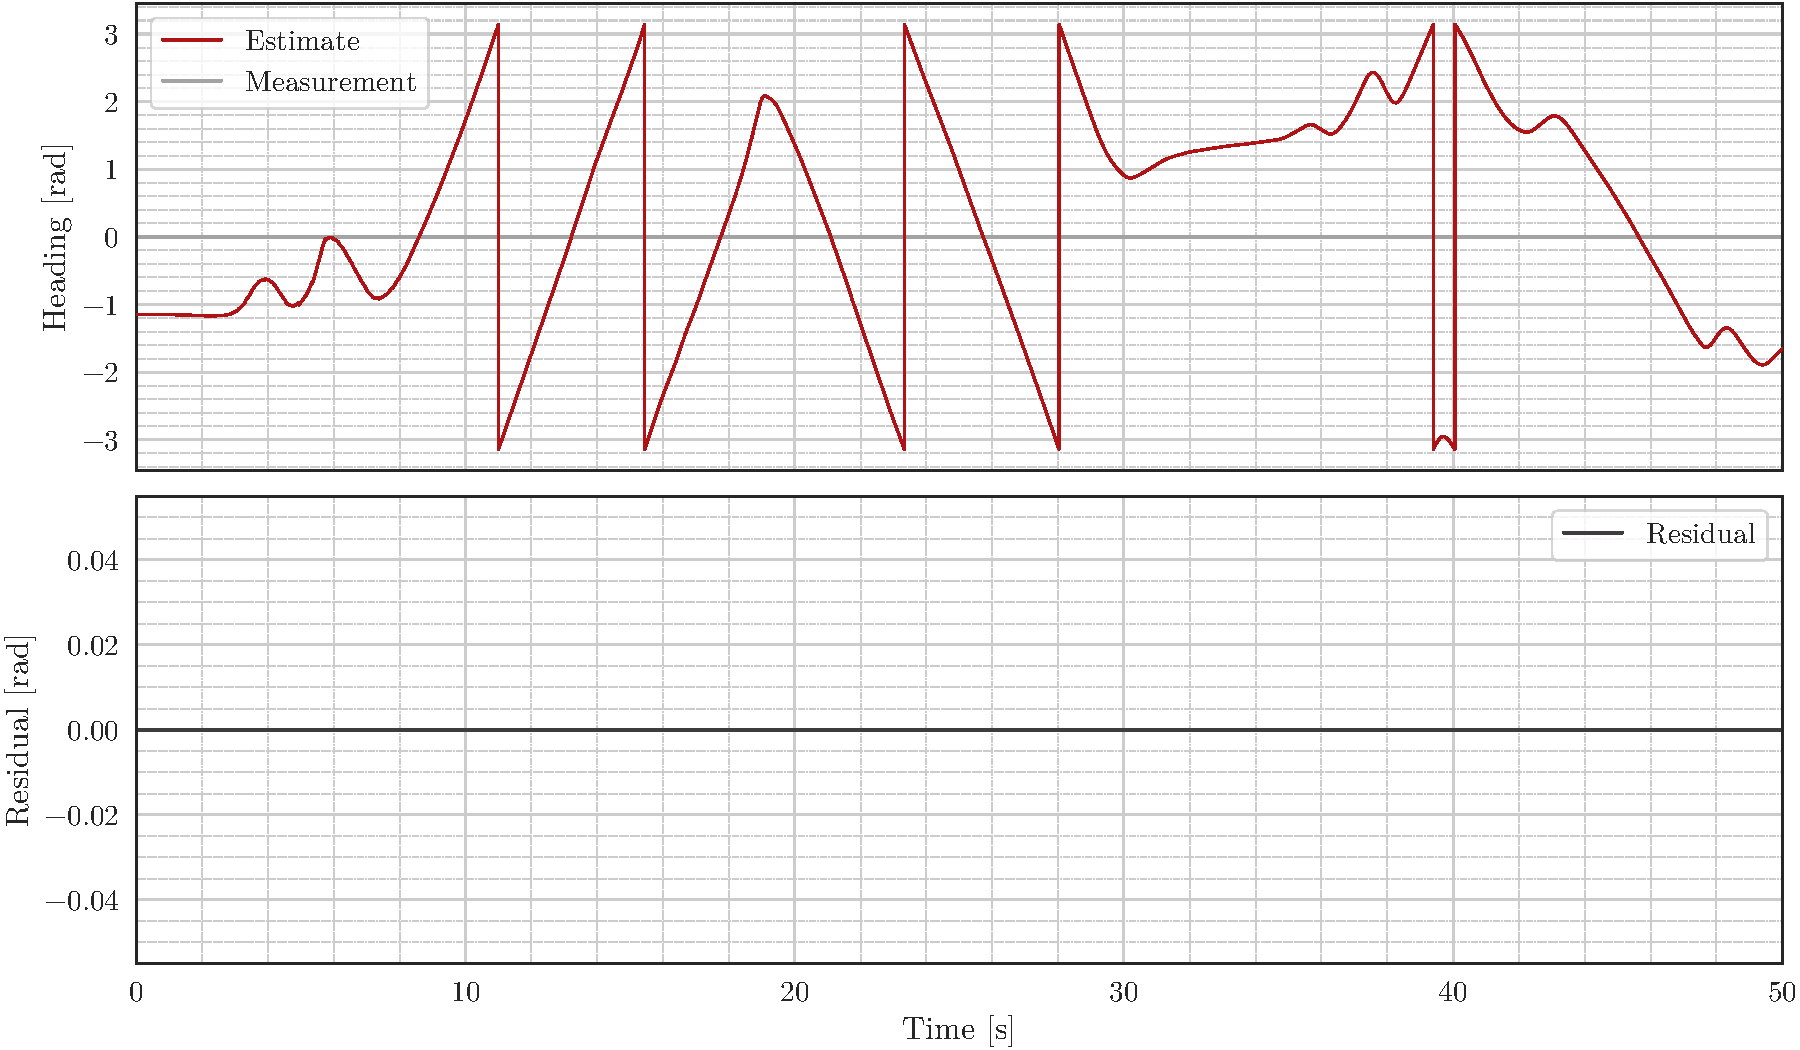
\includegraphics[width=\textwidth]{plot_ekf_full_psi_heading}
\subsection{Yaw rate from IMUs}
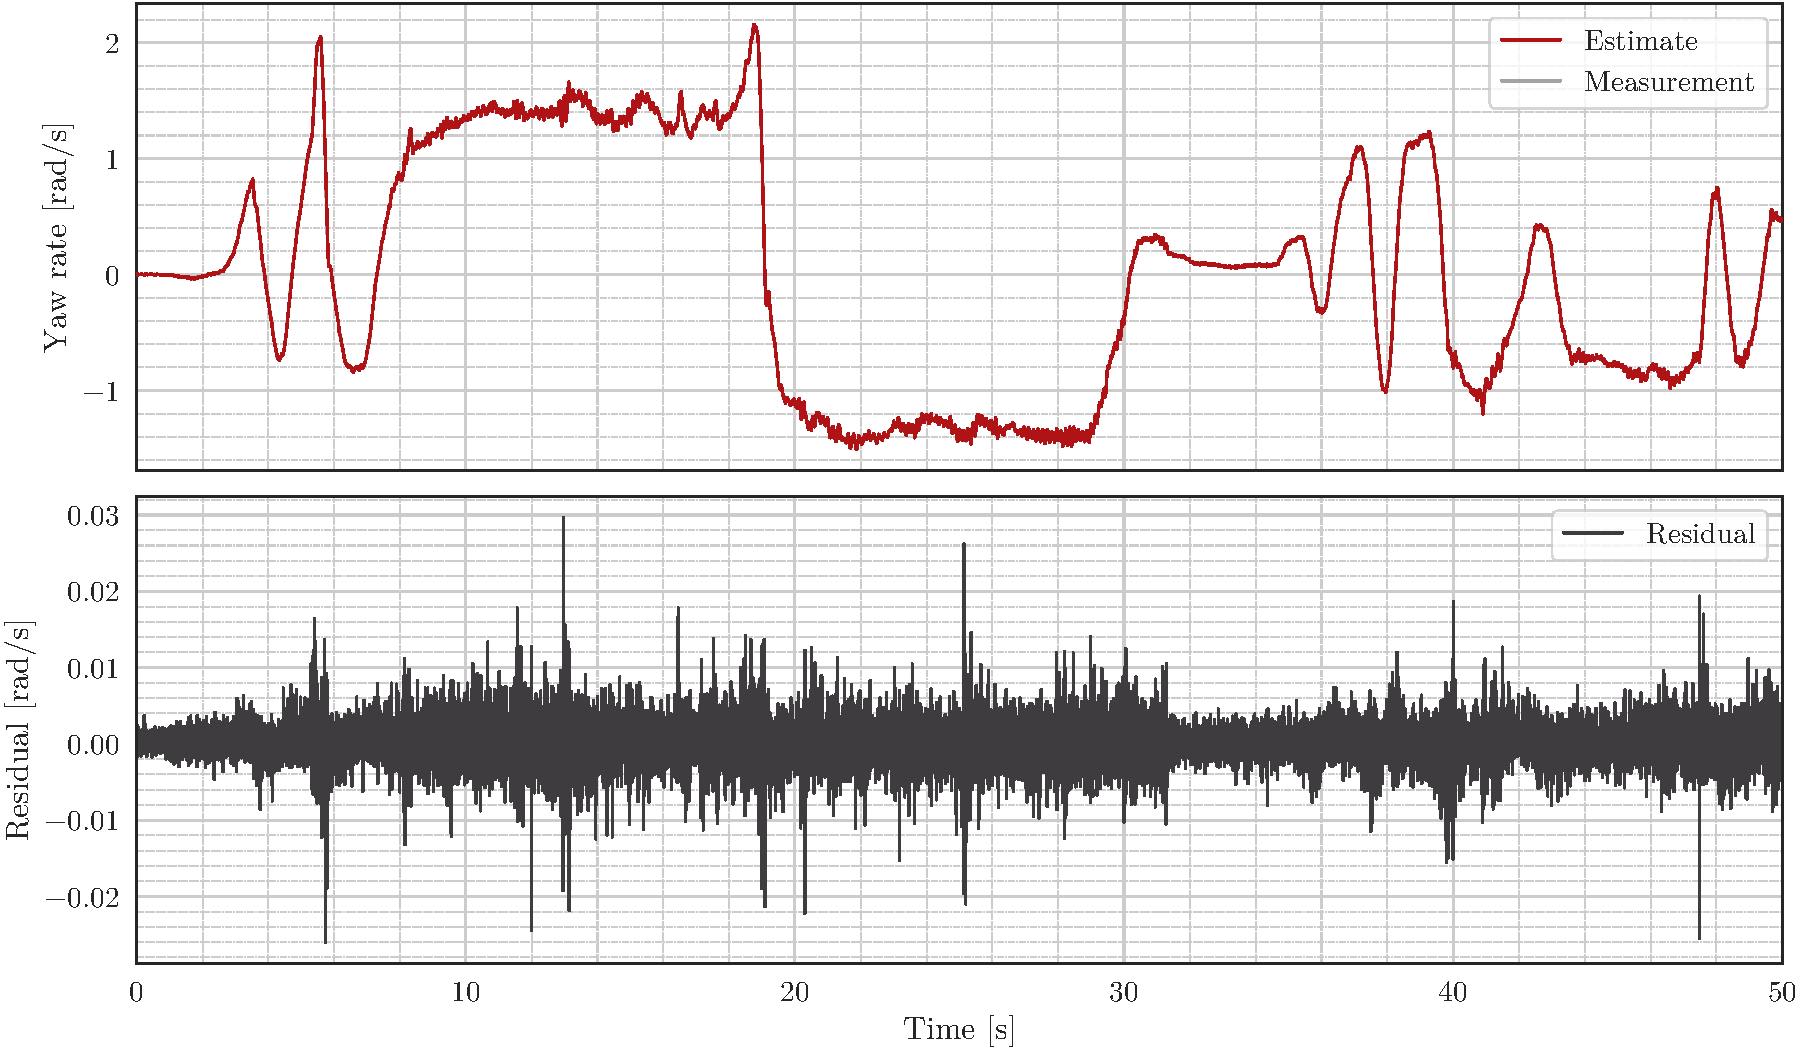
\includegraphics[width=\textwidth]{plot_ekf_full_dpsi}
